\documentclass[10pt,twocolumn,letterpaper]{article}

\usepackage{report}
\usepackage{times}
\usepackage{graphicx}
\usepackage{amsmath}
\usepackage{amssymb}

% Include other packages here, before hyperref.

% If you comment hyperref and then uncomment it, you should delete
% egpaper.aux before re-running latex.  (Or just hit 'q' on the first latex
% run, let it finish, and you should be clear).
\usepackage[pagebackref=true,breaklinks=true,letterpaper=true,colorlinks,bookmarks=false]{hyperref}


%%\reportfinalcopy % *** Uncomment this line for the final submission

\def\reportPaperID{****} % *** Enter the Project Paper ID here
\def\httilde{\mbox{\tt\raisebox{-.5ex}{\symbol{126}}}}

% Pages are numbered in submission mode, and unnumbered in camera-ready
\ifreportfinal\pagestyle{empty}\fi
\begin{document}

%%%%%%%%% TITLE
\title{A Probabilistic Topic Models Based Music Recommendation System
}

\author{Lixuan Zhu\\
Rutgers University-New Brunswick\\
{\tt\small lz306@scarletmail.rutgers.edu}
% For a paper whose authors are all at the same institution,
% omit the following lines up until the closing ``}''.
% Additional authors and addresses can be added with ``\and'',
% just like the second author.
% To save space, use either the email address or home page, not both
\and
Zheng Yu\\
{\tt\small zy120@scarletmail.rutgers.edu}
\and
Yi Zhong\\
{\tt\small yz614@scarletmail.rutgers.edu}
\and
Shihao Su\\
{\tt\small ss2719@scarletmail.rutgers.edu}\\
}

\maketitle
% \thispagestyle{empty}

%%%%%%%%% ABSTRACT
\begin{abstract}
   We will implement a music recommendation system utilizing Probabilistic Topic Models. Specifically, given a song, the system will find a series of similar songs according to features such as metadata, tags and acoustic characteristics.
\end{abstract}

%%%%%%%%% BODY TEXT
\section{Introduction}

%-------------------------------------------------------------------------
Topic Models are a collection of algorithms that finds the underlying topics from a large amount of text documents. According to Blei, each document is a mixture of corpus-wide topics; each topic is a distribution over words and each word is drawn from one of those topics \cite{slides}. When a distribution of topics of the document emerge from topic modeling, we can compute the similarity between two documents by comparing their topic distributions, thus the documents with high similarity to the given document can be recommended to user.
\par
There are two general approaches when designing recommendation systems: collaborative filtering and content-based filtering, each with their strengths and weaknesses. Collaborative filtering utilizes the preferences of existing users and predict whether a specific user will like an item based on the decision of similar users. Music streaming services such as Last.fm utilizes collaborative filtering to recommend songs based on specific user profiles \cite{collaborative}. However, a natural challenge for collaborative filtering methods is the lack of user ratings, also referred to as the “cold start” problem \cite{collaborative}. For example, when a new song is published, there is not enough user rating for the system to know which users will like the song. The other method, content-based filtering, focuses on the similarity of the songs itself. Pandora, another popular music streaming service, utilized the metadata(artist, genre, etc.) and tags to find similar songs given an initial seed song \cite{miami}. Although content-based approaches require very little initial information, it is limited to recommend the songs similar to the original seed since the information about the song is limited.
   \par
   In this project, we take the content-based filtering a step forward. We utilize two probabilistic topic models, latent dirichlet allocation(LDA) and hierarchical dirichlet process(HDP), to discover the similarity between songs and compare their performances. We consider each song as a document and the features of the song as words. It is important to define what we mean by features. Traditional recommendation systems uses the metadata of the song itself and tags by users as measures for similarity. In our model, we incorporate acoustic properties of the music such as pitch, tempo, verses and chords used, mood progression, etc. The timeline API from Gracenote is used to retrieve acoustic properties from the songs\cite{grace}. Collectively, we consider the traditional measures and acoustic properties of the song as features. Thus each feature is a word in the document. The probabilistic topic models process the entire collection of songs as a corpus. The advantage of utilizing acoustic properties is the range of songs recommended can be extended. Songs with similar acoustic properties may not be in the same genre or tagged with similar attributes. The details of the implementation of our models and the challenges of utilizing acoustic properties will be covered in section 3.
   \par
   Another focus of our project is to compare two topic modeling algorithms, LDA and HDP. We plan to analyze the performance of both algorithms in terms of complexity and recommendation result. In comparison, our HDP model is based on LDA and more complex in terms of implementation. However, LDA requires a priori entry of the number of topics in the corpus. How to choose the input value and whether the recommendations are meaningful will be addressed in section 4.


%------------------------------------------------------------------------
\section{Prior Work}
 Blei, Ng, and Jordan specified a popular probabilistic model for discovering latent semantic topics in large collections of text documents in Latent Dirichlet Allocation\cite{lda}. Hu and Saul used symbolic and audio model of music to classify western tonal music in A Probabilistic Topic Model for Music Analysis\cite{ptm}. Hoffman ,Blei and Cook developed a HDP-based way to compute the similarity of songs, which is much faster and better than previous approaches that compare single Gaussian distributions directly\cite{hdp}. Hariri, Mobasher and Burke presented a context-aware music recommender system which infers contextual information based on the most recent sequence of songs liked by the user\cite{context}. Salit, Weinshall and Chechik applied the topic model to model music influence and study properties of influence\cite{influence}. 
\section{Models, Assumptions and Requirements}

\subsection{Word Model of Songs}
In order to find topics from songs with probabilistic topic model, we need to preprocess the audio and metadata of the songs to extract “audio words”. Based on the probabilistic topic model of Diane J. Hu and Lawrence K. Saul\cite{ptm}, our model is defined as follow: 
%\begin{itemize}
%   \item
\par
1. Word list is defined as $u \in$  \{\{metadata\}, \{tag\}, \{pitch\}, \{tempo\}, \{verses\}, \{chords\}, \{mood progression\}\}. Every subset in u(e.g. {metadata}, {tag},etc) will be refined to detailed “audio words” during in the process. Words in different subsets will be weighted as we don’t want artist, genre type of words to have too much contribution to the final results;
%\item
\par
2. A Segment is defined as a  group of words in an unit of time. The words in the nth segment is defined by sgn = {sgn$_{1}$, . . . , sgn$_{L}$, where sgn$_{l}$ is the lth word in the segment.
%\item
\par
3. A song s is defined as a sequence of D segments: s = {sg$_{1}$,...,sg$_{D}$.
%\item
\par
4. The collection of M songs are S = {{s$_{1}$,...,s$_{M}$. 
%\item
\par
5. A topic $\beta \in$  \{1, . . . , K \} is a probability distribution over the elements of word list.  
%\end{itemize}


\subsection{Latent Dirichlet Allocation}
We know that LDA is an unsupervised, probabilistic, generative model for discovering latent semantic topics in large collections of document data. Now we adapt the LDA for songs. Comparing with original LDA, our model treats each song as a “document” and the features of a song as words. Our purpose of modeling is to mining the “topics” in collections of song dataset.
First we have following assumption: Each discovered “topic” is characterized by its own distribution over features. Each song is then characterized as a random mixture of topics indicating the proportion of features each topic over songs\cite{lda}. Our goal is exactly such random mixture of topics, which expresses the meaning and style of a song. By using this, we can compare how similar one song is to another by calculating how similar the corresponding topic mixtures are and recommend similar songs.
 When we do generative process of LDA, we need specify topics we will use first, then calculate the probability of the feature generate by the topic. Finally we use Gibbs sampling to go over all the features. In order to do this, we describe LDA more formally with following notation. Our model suppose each song corresponding with K topics $\beta$$_{1:k}$. The topic proportions for the dth song are d , the topic assignment for dth song are Z$_{d}$, the observed features for song d are W$_{d}$. By using these notation, the joint distribution of the generative process for LDA is shown as equation 1. Then we compute the conditional(posterior) distribution of the topic, which shown as equation 2, and the denominator is the marginal probability of observed corpus. Finally the two distribution will converge and we get what we want. 
\begin{figure}[h]
            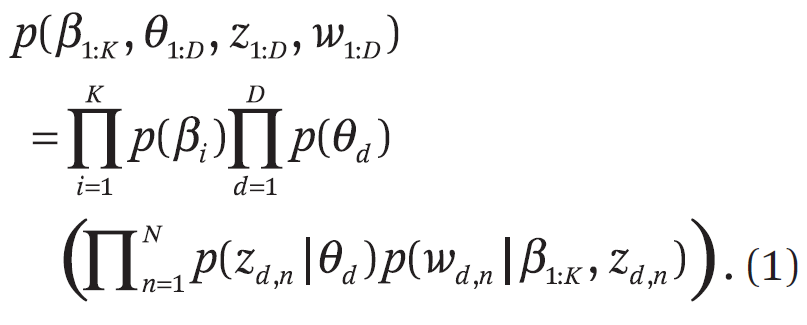
\includegraphics[width=.6\linewidth]{1.jpg}
            \label{fig:graph1}
        \end{figure}

\begin{figure}[h]
            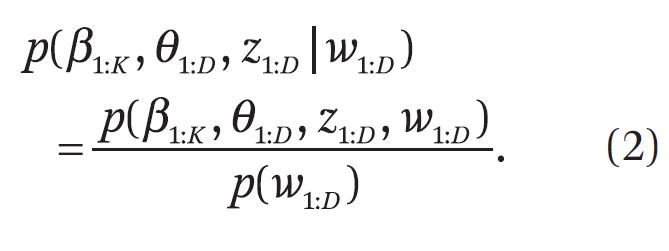
\includegraphics[width=.6\linewidth]{2.jpg}
            \label{fig:graph1}
        \end{figure}
\subsection{Hierarchical Dirichlet Process}
The Hierarchical Dirichlet Process (HDP) is a model of grouped data. We will construct a HDP to model songs represented as a collection of features. The HDP will generate the number of clusters; the clusters here represent the different topics of songs.
Rather than associate each song with a single topic in local, each song is represented as a group of global topics. Thus, each song is represented as a distribution over latent components, but the population of latent components is shared across songs. The HDP model of songs can be generated with the Chinese Restaurant Franchise (CRF). The CRF takes two hyper parameters $\alpha$ and $\gamma$. Each song j has its own CRP, and each feature vector chooses a topic from CRP($\alpha$). If it fit a new distribution, then it chooses a topic for that distribution from a global CRP (with hyper parameter γ) shared by all songs – that is, it either chooses a topic that is already being assigned to some other distributions m with probability proportional to m, or it chooses a new topic with probability proportional to $\gamma$. In this setup, the songs correspond to groups and topics correspond to the factor $\theta$$_{ji}$. We also let $\phi$$_{1}$,$\phi$$_{2}$...$\phi$$_{k}$ denote k random variables distributed according to H; this is the global list of topics. We also introduce variables, $\psi$$_{jt}$, that represent the distribute-specific choice of topics; in particular, $\psi$$_{jt}$ is the topic assigned to distribution t in song j\cite{hdp2}. We put these factors into HDP model and get the formula below.

\begin{figure}[h]
            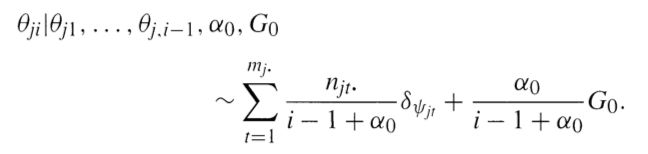
\includegraphics[width=.6\linewidth]{3.jpg}
            \label{fig:graph1}
        \end{figure}


 Finally, we cluster the data with Collapsed Gibbs sampling algorithm in the HDP model. The clusters we get are the specific global topics of all songs. The number of clusters K can be the input of LDA model.

\section{Evaluation}
The goal of our system is to recommend songs for users. Therefore, the most important evaluation will be the accuracy of our recommendation. In other word, are the songs selected by our system satisfy the emotional demands of users? We will evaluate the recommendation result based on feedback from users. 

Moreover, we will implement two algorithms (LDA and HDP) and test them on specific dataset. We used data set from Gracenote, Inc\cite{grace} to extract acoustic features of the songs. To evaluate how our two models fit the data, we need to compare the topics extracted between the two models. LDA requires a priori entry of cluster numbers K. We will input different  K to evaluate the output and decide the range of K for the best output.

\section{Plan}
The project will be finished by early December. The first step is to evaluate the existing implementation of LDA and HDP algorithms and see if any of them can be tweaked to fit our data. This step will be finished by Nov. 6th. The next step will be to explore ways to measure similarities between songs. When we have a distribution of features of the songs, how much weight do we put on each feature and how do we calculate the similarities? This step will be done by Nov. 13th. The third step will be building user interface to interactively make recommendations. This step will be done by Nov. 27th. The last step will be testing the system, evaluating the algorithms and writing project report. This step will be finished by Dec. 3th.

{\small
\bibliographystyle{ieee}
\bibliography{egbib}
}


\end{document}
